% Paper 4: paper 3 (co-author revision) with corrected disclosures, registration details, and verified method details.
% Compile: pdflatex main; bibtex main; pdflatex main; pdflatex main.
\documentclass[conference]{IEEEtran}
\IEEEoverridecommandlockouts
\usepackage{iftex}
\ifXeTeX
  \usepackage{fontspec}
  \setmainfont{texgyretermes}[Extension=.otf, UprightFont=*-regular, BoldFont=*-bold, ItalicFont=*-italic, BoldItalicFont=*-bolditalic]
\else
  \usepackage[T1]{fontenc}
\fi
\usepackage{cite}
\usepackage{amsmath,amssymb}
\usepackage{graphicx}
\usepackage{booktabs,array,tabularx}
\usepackage{xcolor}
\usepackage{url}
\usepackage{tikz}
\usetikzlibrary{positioning,arrows.meta,fit,calc}
\usepackage{algorithm}
\usepackage{algpseudocode}
\usepackage[hidelinks]{hyperref}
\hypersetup{pdftitle={Do LLM Agents Verify Their Data? Available vs. Enforced Checks in Data Mining},pdfauthor={Ahsan Shahid; Mohammed Muzakkiruddin Ahmed; Hadi Rashid; Abdelrahman Elfikky; John R. Talburt},pdfsubject={Available versus enforced data verification in LLM-agent data mining},pdfkeywords={data mining, data quality, data provenance, LLM agents, verification, multi-agent systems}}
\newcommand{\sys}[1]{\textsf{#1}}
\newcommand{\vcr}{\mathrm{VCR}}
\newcommand{\code}[1]{\texttt{#1}}
\newcolumntype{Y}{>{\raggedright\arraybackslash}X}
\begin{document}

\title{Do LLM Agents Verify Their Data?\\ Available vs.\ Enforced Checks in Data Mining}
\author{\IEEEauthorblockN{Ahsan Shahid, Mohammed Muzakkiruddin Ahmed, Hadi Rashid, Abdelrahman Elfikky, and John R. Talburt}
\IEEEauthorblockA{Center for Entity Resolution and Information Quality\\
University of Arkansas at Little Rock, Little Rock, AR 72204, USA\\
\{axshahid, mmohammed6, harashid, aelfikky1, jrtalburt\}@ualr.edu}}
\maketitle

\begin{abstract}
A data-mining pipeline can produce plausible predictions while using an unauthorized file, losing records, or mixing units. We investigate whether large language model (LLM) agents use available data-verification operations and whether enforcing checks improves pipeline reliability. A controlled benchmark combines 36 classification and regression tasks from six dataset families with declared and hidden defects. Seven systems---a rule-based workflow, two single-agent configurations, and four three-agent configurations---share data-processing tools, candidate models, and resource limits. An independent evaluator checks submitted workflows against hidden references. The protocol was frozen before evaluation and registered; the main, replication, and refusal experiments comprise 8,352 runs. On silent content drift, the ungated single agent and team used a hash-verifying load in only 1 and 12 of 108 runs, compared with 104--107 for provenance-gated agents. However, the primary comparison between the fully gated and ungated teams showed no overall improvement: $+0.1$ percentage points (95\% confidence interval: $-11.1$ to $+9.9$). Benefits on hidden defects were offset by a range check that rejected correct data in two of 18 family--repetition blocks. The fully gated team also completed fewer verified pipelines than the gated single agent, and a second model reproduced the primary pattern. These findings distinguish access to verification from its actual use: enforcement can address observable defects, but unreliable checks can turn correct workflows into failures.
\end{abstract}
\begin{IEEEkeywords}
data mining, data quality, data provenance, LLM agents, verification, multi-agent systems
\end{IEEEkeywords}

\section{Introduction}
Imagine a predictive-maintenance pipeline that selects the approved sensor dataset, trains a model, and returns convincing predictions. Its catalog entry names the correct file version, but the file itself has been silently replaced. Nothing in the values looks unusual. Unless the pipeline checks the stored content against the authorized hash, its apparent success conceals a data-handling failure. This is the distinction at the center of this study: completing an analysis is not the same as verifying the data used to produce it.

The problem predates LLM agents. Work on technical debt in machine learning identified data dependencies as a continuing source of system risk~\cite{sculley2015debt}. Large-scale verification and production data-validation systems subsequently made many checks executable~\cite{schelter2018deequ,polyzotis2019datavalidation}. More recently, Kapoor and Narayanan documented how data leakage undermines reproducibility in machine-learning-based science~\cite{kapoor2023leakage}. As agents take responsibility for finding, cleaning, joining, and modeling data, these established concerns become questions about autonomous behavior: will an agent perform a check simply because the operation is available?

Data-science benchmarks have established important evidence about agents' ability to complete realistic analyses~\cite{hu2024infiagent,jing2025dsbench,chan2025mlebench}. However, a correct answer or strong predictive score does not by itself establish that source selection, record matching, unit conversion, and model validation were correct. An audit of agentic data-science workflows found methodological failures even when downstream performance appeared satisfactory~\cite{li2026silent}. Evaluating the process therefore complements, rather than replaces, evaluating the final result.

Two common approaches are to ask agents to check their work and to distribute responsibilities across specialized agents. Neither guarantees verification. Studies of intrinsic self-correction report limitations without external feedback~\cite{huang2024selfcorrect}, whereas tool-grounded feedback can support correction~\cite{gou2024critic}. Enforcing an executable check is a stronger intervention, but its value depends on the rule: a check that incorrectly rejects valid data can prevent a sound pipeline from completing.

We study this trade-off through four research questions. \textbf{RQ1:} Do agents use an available verification operation without enforcement? \textbf{RQ2:} Does enforcing quality and provenance checks improve verified completion relative to an ungated team (primary hypothesis H1)? \textbf{RQ3:} What do quality and provenance checks contribute separately and jointly, and which defects account for their effects (H2)? \textbf{RQ4:} Under common resource limits, how does a fully gated team compare with a gated single agent (H3) and a rule-based workflow on declared defects (H4)?

Development pilots motivated a distinction between \emph{declared defects}, whose remedies are stated, and \emph{hidden defects}, which violate a stated requirement without announcing the violation. When all defects and remedies were explicit, every system, including the rule-based workflow, solved 95--100\% of pilot tasks. Hidden defects were therefore added to examine verification and recovery rather than specification following alone.

The study makes three contributions. First, it provides a benchmark of 36 tasks with an independent corruption ledger, hidden-reference evaluation, and an oracle solvability check. Second, it separates planning structure from enforced quality and provenance checks while keeping the hash-verifying operation available to all systems. Third, it reports 8,352 evaluation runs under a frozen protocol, including the unsupported primary hypothesis, defect-specific benefits, and a false-alarm failure mode of enforcement. The contribution is a controlled evaluation framework and empirical evidence, not a new predictive-learning algorithm.

\section{Related Work}
\label{sec:related}
\subsection{Data-science agents and their evaluation}
InfiAgent-DABench supports automatic evaluation of data-analysis questions~\cite{hu2024infiagent}; DSBench adds realistic analysis and modeling tasks~\cite{jing2025dsbench}; and MLE-bench evaluates machine-learning engineering against Kaggle competition outcomes~\cite{chan2025mlebench}. DABstep emphasizes multi-step analysis~\cite{egg2025dabstep}, Spider~2.0 enterprise SQL workflows~\cite{lei2025spider2}, and the Data Agent Benchmark heterogeneous data sources~\cite{ma2026dab}. These benchmarks establish complementary measures of task capability, rather than interchangeable success rates.

Agent architectures also offer useful building blocks. DS-Agent uses case-based reasoning~\cite{guo2024dsagent}, Data Interpreter organizes interdependent work through task graphs~\cite{hong2024datainterpreter}, and DS-STAR addresses heterogeneous formats and open-ended queries~\cite{nam2025dsstar}. Our study does not rank these end-to-end systems. It uses a bounded environment to isolate planning and verification choices. This complements the methodological audit of Li et~al.~\cite{li2026silent}, which demonstrates why accurate predictions and executable code are insufficient evidence of sound data science.

\subsection{Data quality, repair, and provenance}
Production data validation~\cite{polyzotis2019datavalidation} and Deequ-style verification~\cite{schelter2018deequ} show how data expectations can become executable checks. HoloClean studies probabilistic repair~\cite{rekatsinas2017holoclean}, while mlinspect examines distribution changes introduced by pipeline operations~\cite{grafberger2021mlinspect}. Provenance provides a complementary view: PROV-DM describes data entities, activities, and derivations~\cite{w3c2013provdm}, and Vamsa tracks provenance in data-science scripts~\cite{namaki2020vamsa}. We draw on these ideas to distinguish checking data properties from checking source identity and transformation history.

Recent agentic work extends this foundation. DataGovBench evaluates end-to-end data-governance workflows~\cite{liu2025datagovbench}. Fadlallah reports trade-offs among detection, evidence grounding, and conservative repair in reference-free cleaning~\cite{fadlallah2026cleaning}; Parmar et~al. find that debate can help error detection but can also harm generation~\cite{parmar2026debate}. A context-aware assessment framework validates the feasibility of agent-generated rules before executing them~\cite{fadlallah2026dqa}. These studies motivate examining the quality of the checking mechanism, not only whether an agent has one.

\subsection{Verification and multi-agent coordination}
SARC-DQ shows that metadata-aware gates can recover losses on defects covered by their predicates~\cite{besanson2026sarcdq}; related work explains how remediation by one gate can affect another~\cite{besanson2026onegate}. RITE identifies recognition, use of a verification path, and integration of evidence as separate bottlenecks~\cite{zhang2026rite}. LIMBO distinguishes model behavior from guarantees provided by tool contracts~\cite{li2026limbo}. In coding, completion gates and independent review can improve outcomes, with different resource costs~\cite{zhang2026rethinking}, while ContextCov converts documented constraints into executable checks~\cite{sharma2026contextcov}. Verification prompts can also reduce reliance on corrupted tool outputs~\cite{yang2026overreliance}. These findings motivate our comparison, but their effects should not be assumed to transfer unchanged to data mining.

ReAct provides a tool-interaction pattern~\cite{yao2023react}, while AutoGen and MetaGPT support role-based coordination~\cite{wu2023autogen,hong2024metagpt}. Evidence on teams is mixed. Matched-budget reasoning studies find no consistent team advantage~\cite{tran2026single,dylan2026equalcost}; broader comparisons identify both successful configurations and substantial overhead~\cite{fu2026moreagents,jwalapuram2026illusion}. Benefits depend on task structure and coordination design~\cite{kim2025scaling}, and verification remains a documented failure category~\cite{cemri2025mas}. Accordingly, our conclusions concern the tested three-role design, not multi-agent systems in general.

\begin{table*}[t]
\caption{Positioning against representative research. The final column describes the focus of this study, not a claim that previous work lacks all related capabilities.}
\label{tab:related}
\centering\footnotesize
\begin{tabularx}{\textwidth}{@{}p{0.24\textwidth}YY@{}}
\toprule
Research line & Established contribution & Focus of the present comparison \\
\midrule
Data-science benchmarks~\cite{jing2025dsbench,chan2025mlebench,egg2025dabstep,ma2026dab} & Realistic analysis, modeling, and multi-source task evaluation. & Hidden-reference checks of source authority, records, joins, units, and aggregates, beyond final-answer scoring. \\
DataGovBench and workflow audits~\cite{liu2025datagovbench,li2026silent} & Governance evaluation and identification of methodological failures. & Paired interventions on verification availability versus enforced checks within one bounded task environment. \\
Validation and provenance systems~\cite{schelter2018deequ,polyzotis2019datavalidation,w3c2013provdm,namaki2020vamsa} & Executable data constraints and traceable transformations. & Quality and provenance as separate experimental factors, including their interaction and false alarms. \\
SARC-DQ, RITE, and verification harnesses~\cite{besanson2026sarcdq,zhang2026rite,zhang2026rethinking} & Evidence-integrity gates, silent-error diagnosis, and verification placement. & Data-mining workflows with the same verified-load operation available to every system. \\
Compute-aware agent comparisons~\cite{tran2026single,fu2026moreagents,kim2025scaling} & Analysis of coordination benefits, task dependence, and resource costs. & Rule-based, single-agent, and three-role systems under common resource ceilings and independent evaluation. \\
\bottomrule
\end{tabularx}
\end{table*}

\subsection{Research opportunity}
Table~\ref{tab:related} places the study at the intersection of these lines of work. Its distinctive feature is their combination: explicit data-handling outcomes; an identically documented verifying load; separate quality and provenance interventions; conventional and agentic baselines; and an analysis plan frozen before evaluation. Rather than claiming that verification or process-based evaluation is new, we ask how these elements interact in a controlled data-mining setting.

\section{Methodology}
\label{sec:method}
\subsection{Controlled design and rationale}
We use a paired experiment: systems receive the same task instances, data-processing operations, candidate models, and resource ceilings. Pairing reduces variation caused by task difficulty and supports direct comparisons of the tested system configurations. Common ceilings prevent a team from receiving a separate budget for each role; they do not imply equal realized compute or runtime. The intervention also includes gate feedback and check-related instructions, so its effect cannot be attributed to blocking alone.

Hypotheses, analysis choices, and resource limits were fixed before the evaluation runs and stored in a hashed protocol record, following the rationale of preregistration~\cite{nosek2018prereg}. The frozen package was registered on OSF (DOI 10.17605/OSF.IO/BN6VA) on 13 Nov.\ 2026 (UTC), after the freeze and while the evaluation runs were in progress, before any formal result was analyzed. Software, rather than human or LLM grading, determines the outcome. This makes the scoring rules explicit, although their validity still depends on the evaluator and task specification.

\subsection{Datasets and task construction}
\label{sec:bench}
Table~\ref{tab:data} summarizes the six dataset families. D1--D4 are public UCI datasets distributed under CC~BY~4.0. They cover classification and regression with documented attributes; AI4I~2020 is synthetic~\cite{matzka2020ai4i}, and Energy Efficiency describes simulated buildings~\cite{tsanas2012energy}. D5 and D6 use seeded relational generators to provide newly generated instances and reduce dependence on potentially familiar public datasets. This does not establish that the broader task patterns are absent from model training.

Each family has six templates: single-source modeling (T1); two-table and three-table integration (T2, T3); harmonization of documented units (T4); selection of the authorized source version (T5); and per-record aggregation of child readings (T6). The resulting 36 tasks test different points at which data handling can fail. Tables are divided into 20 shards per partition. Every system receives a contract specifying the target, allowed and excluded features, source versions, keys, units, aggregation rules, plausible ranges, and resource budget.

\begin{table}[t]
\caption{Dataset families. Row counts describe each source dataset.}
\label{tab:data}
\centering\footnotesize\setlength{\tabcolsep}{4pt}
\begin{tabular}{@{}llrl@{}}
\toprule
ID & Source & Rows & Target \\
\midrule
D1 & AI4I 2020~\cite{uci601ai4i} & 10,000 & Failure (binary) \\
D2 & Steel Plates Faults~\cite{uci198steel} & 1,941 & Fault (7 classes) \\
D3 & Concrete Strength~\cite{uci165concrete,yeh1998concrete} & 1,030 & Strength (regression) \\
D4 & Energy Efficiency~\cite{uci242energy} & 768 & Heating load (regr.) \\
D5 & Synthetic machinery & 10,000 & Failure (binary) \\
D6 & Synthetic process & 9,000 & Output (regression) \\
\bottomrule
\end{tabular}
\end{table}

\subsection{Declared and hidden defects}
Tier~1 comprises a clean condition and declared defects with stated remedies: missing or string-encoded numbers affecting 5\% or 20\% of cells; duplicated or aliased keys at 5\% or 20\%; and changed representations or stale sources affecting one quarter of shards. Tier~2 retains the contract but does not disclose the injected violation (Table~\ref{tab:tier2}). X2 introduces key variants that disrupt matching. X3 places shards in an undeclared unit representation. X4 replaces authorized file contents while leaving the catalog's version and hash unchanged; a correct replica remains available.

X4 values remain plausible. Within this construction, recomputing content hashes is the reliable way to distinguish the altered file from its authorized replica. A hash verifies agreement with a trusted reference, not whether that reference is scientifically correct. Every system receives documentation for the general repair operations in both tiers. Pilot severity was selected by a rule fixed in advance: choose the level whose baseline success rate is closest to 0.5, avoiding an uninformative ceiling or floor~\cite{wang2026dbe}. Formal evaluation uses the frozen levels rather than retuning them to the final results.

\begin{table}[t]
\caption{Tier~2 defects. Bold values are the frozen severity levels. Q and P denote quality and provenance checks.}
\label{tab:tier2}
\centering\footnotesize\setlength{\tabcolsep}{3pt}
\begin{tabularx}{\columnwidth}{@{}lp{0.25\columnwidth}p{0.23\columnwidth}Y@{}}
\toprule
ID & Candidate severity & Check & Repair operation \\
\midrule
X2 & 5\% / \textbf{10\%} / 20\% of keys & Record coverage (Q) & \code{\scriptsize normalize\_key} \\
X3 & \textbf{1} / 2 / 4 of 20 shards & Value ranges (Q) & \code{\scriptsize infer\_representation} \\
X4 & 1 / \textbf{2} / 4 of 20 shards & Content hash (P) & Verified load policy \\
\bottomrule
\end{tabularx}
\end{table}

\subsection{Independent evaluation and solvability}
The generator stores a ledger of injected changes outside the agent environment. A separate evaluator replays the submitted workflow on hidden test data and compares it with an independent reference. It checks the target, source authority, excluded features, records, joins, units, and aggregates, using absolute tolerance $10^{-8}$ and relative tolerance $10^{-6}$. It also checks training-only preprocessing and valid predictions for every hidden record. A submission succeeds only when all required predicates pass; a strong predictive score cannot compensate for a failed data-handling check.

Known-verdict fixtures tested the evaluator before runs began. Following the emphasis on solvability in the Agentic Benchmark Checklist~\cite{zhu2025abc}, an oracle solver reproduced the hidden reference on all 324 formal Tier~2 instances before the freeze. This establishes solvability under the reference construction, not that every gate accepts the correct solution. That distinction is important because the later range-check failures concern gate validity rather than task solvability.

\subsection{Systems and comparison structure}
\label{sec:systems}
Table~\ref{tab:systems} defines the seven systems. \sys{F} is a rule-based workflow derived from the declared contract; it uses both gates but does not adapt beyond its programmed repairs. \sys{S0} and \sys{SQP} use one agent without or with both gates. The three-role team has four configurations: neither gate (\sys{M0}), quality only (\sys{MQ}), provenance only (\sys{MP}), and both (\sys{MQP}). This $2\times2$ team design separates gate main effects from their interaction. The single-agent comparison tests coordination while retaining both gates, and \sys{F} tests whether adaptive planning adds value on explicitly specified repairs.

\begin{table}[t]
\caption{System configurations. Common data tools include the verified-load policy; gated systems additionally expose check tools and enforce their active predicates.}
\label{tab:systems}
\centering\footnotesize\setlength{\tabcolsep}{5pt}
\begin{tabular}{@{}lllcc@{}}
\toprule
System & Planner & LLM & Quality & Provenance \\
\midrule
\sys{F} & Fixed rules & No & Yes & Yes \\
\sys{S0} & Single agent & Yes & -- & -- \\
\sys{SQP} & Single agent & Yes & Yes & Yes \\
\sys{M0} & Three-role team & Yes & -- & -- \\
\sys{MQ} & Three-role team & Yes & Yes & -- \\
\sys{MP} & Three-role team & Yes & -- & Yes \\
\sys{MQP} & Three-role team & Yes & Yes & Yes \\
\bottomrule
\end{tabular}
\end{table}

\section{System Design and Algorithm}
\label{sec:architecture}
\subsection{Architecture and end-to-end workflow}
Figure~\ref{fig:arch} separates the components responsible for planning, execution, enforcement, and evaluation. The \emph{task layer} exposes the contract, catalog, and training and validation data, while retaining test labels, the corruption ledger, and reference features outside the agent environment. This boundary prevents the planner from consulting the answers used to judge its submission.

The \emph{planning layer} is either the fixed workflow, a single tool-using agent, or a coordinator working with a data manager and mining agent. Agentic configurations follow a ReAct-style action--observation loop~\cite{yao2023react}. Team roles communicate through a shared blackboard, consistent with role-based agent frameworks~\cite{wu2023autogen,hong2024metagpt}. The coordinator delegates work and alone may submit. The shared budget makes coordination consume the same allowance as other reasoning and tool use.

The \emph{execution layer} provides bounded operations: source listing, inspection, profiling, read-only DuckDB queries~\cite{raasveldt2019duckdb}, feature materialization, model evaluation, submission, and abstention. Feature materialization executes a validated declarative graph whose operations include loading, parsing, unit conversion, alias mapping, key normalization, representation inference, de-duplication, joins, and aggregation. The modeling tool evaluates six fixed scikit-learn pipelines~\cite{pedregosa2011sklearn}. Restricting operations improves comparability and enables replay, but narrows the study relative to unrestricted code-writing agents.

\emph{Trusted wrappers} record provenance and account for tokens, model and tool calls, and active time. The \emph{gate layer} applies the active quality and provenance predicates and returns diagnostic feedback. Quality checks concern required columns, excluded features, key uniqueness, record coverage, ranges, unit conversion, and aggregates. Provenance checks concern authority, versions, recomputed hashes, column lineage, and training-data fit scope. Their design draws on data validation and provenance practice~\cite{polyzotis2019datavalidation,schelter2018deequ,w3c2013provdm}. A failed active gate blocks submission, but an agent can revise its workflow within the repair limit.

Finally, the \emph{independent evaluator} replays an accepted submission on hidden data and produces the verified-completion outcome. Thus, gate passage is an intermediate condition, not the outcome itself. The complete path is contract inspection, graph construction, materialization, checking and possible repair, model selection, submission, and hidden evaluation. Separating these responsibilities makes it possible to distinguish skipped checks, incorrect repairs, false alarms, and evaluator failures.

\begin{figure*}[t]
\centering
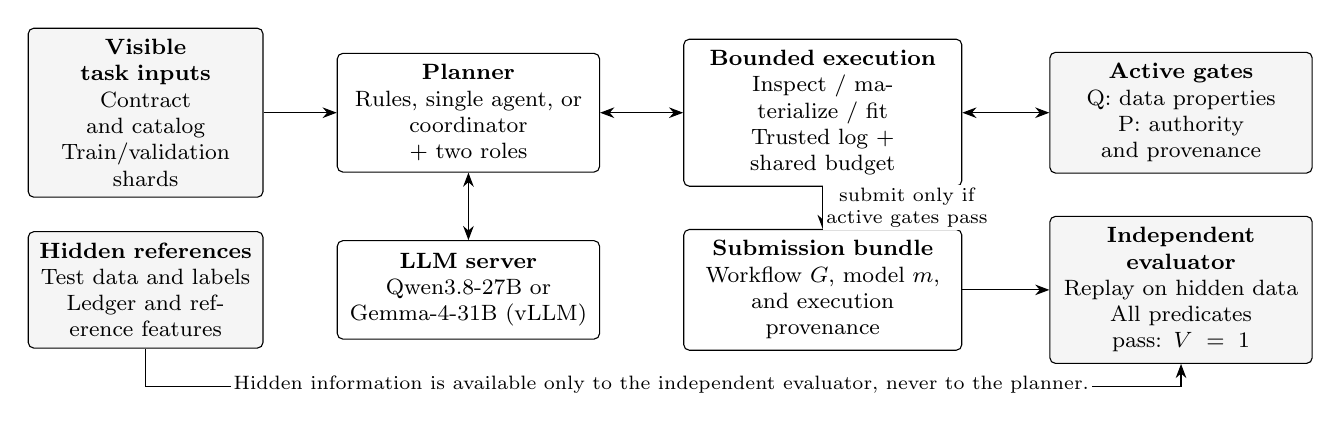
\begin{tikzpicture}[font=\footnotesize, >={Stealth[length=1.8mm]},
 box/.style={draw,rounded corners=2pt,align=center,inner sep=4pt,minimum height=1.25cm},
 lab/.style={font=\scriptsize,align=center,fill=white,inner sep=1pt}]
\node[box,text width=2.7cm,fill=gray!8] (visible) at (0,0) {\textbf{Visible task inputs}\\Contract and catalog\\Train/validation shards};
\node[box,text width=3.05cm] (planner) at (4.1,0) {\textbf{Planner}\\Rules, single agent, or\\coordinator + two roles};
\node[box,text width=3.25cm] (tools) at (8.6,0) {\textbf{Bounded execution}\\Inspect / materialize / fit\\Trusted log + shared budget};
\node[box,text width=3.05cm,fill=gray!8] (gates) at (13.15,0) {\textbf{Active gates}\\Q: data properties\\P: authority and provenance};
\node[box,text width=2.7cm,fill=gray!8] (hidden) at (0,-2.25) {\textbf{Hidden references}\\Test data and labels\\Ledger and reference features};
\node[box,text width=3.05cm] (model) at (4.1,-2.25) {\textbf{LLM server}\\Qwen3.8-27B or\\Gemma-4-31B (vLLM)};
\node[box,text width=3.25cm] (bundle) at (8.6,-2.25) {\textbf{Submission bundle}\\Workflow $G$, model $m$,\\and execution provenance};
\node[box,text width=3.05cm,fill=gray!8] (eval) at (13.15,-2.25) {\textbf{Independent evaluator}\\Replay on hidden data\\All predicates pass: $V=1$};
\draw[->] (visible) -- (planner);
\draw[<->] (planner) -- (tools);
\draw[<->] (tools) -- (gates);
\draw[<->] (planner) -- (model);
\draw[->] (tools) -- node[lab,right]{submit only if\\active gates pass} (bundle);
\draw[->] (bundle) -- (eval);
\draw[->] (hidden.south) -- ++(0,-0.48) -| (eval.south);
\node[lab] at (6.55,-3.46) {Hidden information is available only to the independent evaluator, never to the planner.};
\end{tikzpicture}
\caption{System architecture and trust boundaries. All systems share bounded data operations, including the hash-verifying load. Active gates return feedback and block invalid submissions. The rule-based planner does not call the LLM server; all agent roles share one resource budget. The evaluator remains separate from both the planner and the enforcement layer.}
\label{fig:arch}
\end{figure*}

\subsection{Formal representation and verification policies}
A task instance is $I=(C,K,D,H)$: contract $C$, source catalog $K$, visible training and validation data $D$, and hidden evaluation information $H$. A candidate solution comprises a declarative workflow $G$ and candidate model $m$. Each load node specifies a table and policy $\rho$. For authorized version $v^\star$ and shard hash $h_s^\star$, the ordinary \code{authoritative} policy selects files whose catalog metadata match these declarations. The \code{authoritative\_verified} policy additionally requires
\begin{equation}
\mathrm{SHA256}(f_s)=h_s^\star,
\label{eq:hash}
\end{equation}
where $f_s$ is the stored shard content. The difference is checking the bytes rather than trusting the catalog entry.

Let $\mathcal{S}\subseteq\{Q,P\}$ be the active gate set and $\pi$ the trusted provenance log. A candidate may pass the gate layer only when
\begin{equation}
\mathrm{Pass}_{\mathcal{S}}(G,D,\pi)=
\bigwedge_{g\in\mathcal{S}}\;\bigwedge_j g_j(G,D,\pi)=1.
\label{eq:gate}
\end{equation}
The conjunction is vacuously true for an ungated system, although ordinary tool validity checks still apply. A failing gate returns its predicates for diagnosis; it does not itself establish which repair will succeed. The evaluator independently defines
\begin{equation}
V(I,G,m)=\prod_j\phi_j(G,m;H)\in\{0,1\},
\label{eq:v}
\end{equation}
with $V=0$ for abstention or an exhausted budget. VCR is the proportion of runs with $V=1$. It measures compliance with the specified data-handling requirements, not unrestricted scientific correctness or predictive superiority.

For RQ1, verification uptake is the proportion of runs that pass at least one graph containing a verified-load node to \code{materialize\_features}. It includes attempted intermediate graphs, not only the final submission. Uptake and verified completion are therefore distinct: using a check does not guarantee that all other requirements are satisfied.

\subsection{Execution and repair algorithm}
Algorithm~\ref{alg:run} presents the control flow described by the study. Its inputs are the visible instance, active gates, and shared limits; its outputs are a submission bundle or a termination status. The controller obtains a JSON action, executes the requested operation, returns observations, and repeats. Three consecutive invalid actions terminate the run. After a materialization or submission failure, at most $R=2$ repair materializations are permitted. Once the limit is reached, the controller reports this condition rather than silently granting more repairs.

In the team, delegation invokes the selected specialist for at most 12 steps, charging every role to the same budget. Specialists return observations through the shared state, and only the coordinator submits. \sys{F} instead constructs a fixed graph from $C$ and $K$, uses ordinary authoritative loads and declared repairs, and either submits after both gates pass or abstains. Consequently, making a verified policy available does not cause the rule-based baseline to use it automatically.

\begin{algorithm}[t]
\caption{Bounded agentic workflow with optional enforced gates}
\label{alg:run}
\footnotesize
\begin{algorithmic}[1]
\Require Visible instance $(C,K,D)$; gate set $\mathcal{S}$; budget $B$; $R=2$
\Ensure Submission $(G,m)$, abstention, or failure status
\State $h\gets$ task text from $C,K$; $r\gets0$; $\mathit{failed}\gets\textbf{false}$
\While{$B$ is not exhausted}
  \State $a\gets\textsc{NextAction}(h)$ \Comment{JSON; charge model use}
  \If{$a$ is invalid}
    \State Handle invalid action; stop after three consecutive failures
    \State \textbf{continue}
  \EndIf
  \If{$a=\code{abstain}(\mathit{reason})$}
    \State \Return $\textsc{Abstained}(\mathit{reason})$
  \ElsIf{$a=\code{delegate}(\mathit{role},\mathit{task})$}
    \State $o\gets$ specialist result (team only; at most 12 steps)
    \State Charge specialist actions to the same $B$
  \ElsIf{$a=\code{materialize\_features}(G)$}
    \If{$\mathit{failed}$ and $r=R$}
      \State $o\gets$ ``repair limit reached''
    \Else
      \If{$\mathit{failed}$} \State $r\gets r+1$ \EndIf
      \State Execute $G$ on $D$; record operations in $\pi$
      \State $o\gets$ materialization summaries and active gate verdicts
      \State $\mathit{failed}\gets$ execution error or any failed active gate
    \EndIf
  \ElsIf{$a=\code{submit}(G,m)$}
    \If{$\mathrm{Pass}_{\mathcal{S}}(G,D,\pi)=0$}
      \State $o\gets$ failing checks; $\mathit{failed}\gets\textbf{true}$
    \Else
      \State Refit $m$ on training and validation data
      \State \Return $\textsc{Submitted}(G,m)$ \Comment{Coordinator only in a team}
    \EndIf
  \Else
    \State $o\gets$ result of a read-only tool or \code{fit\_evaluate}
  \EndIf
  \State Account for tool use and time; append $(a,o,\text{remaining }B)$ to $h$
\EndWhile
\State \Return $\textsc{BudgetExceeded}$
\end{algorithmic}
\end{algorithm}

The algorithm describes orchestration rather than introducing a new learning method. During candidate selection, each pipeline, including its preprocessing, is fitted on the training partition only and scored on validation data. At submission, the selected pipeline, again including its preprocessing, is refitted on training plus validation data; hidden test data remain outside the planning loop. The evaluator checks both fit scopes.

\section{Experimental Setup and Statistical Analysis}
\label{sec:setup}
\subsection{Models, resource limits, and experiments}
Backbone A is \code{Qwen/Qwen3.8-27B}~\cite{qwen2026qwen38}; backbone B is \code{google/gemma-4-31B-it}~\cite{google2026gemma4}. Both are revision-pinned open models served through vLLM~\cite{kwon2023vllm} on one NVIDIA RTX PRO 6000 GPU. Settings are temperature 0.2, a 16,384-token context, reasoning mode disabled, and JSON actions. Each run is limited to 300,000 tokens, 48 model calls, 40 tool calls, six model evaluations, two repair cycles, and 600\,s of active time. The token ceiling follows a rule fixed before the pilots.

The experiment identifiers follow the frozen study records. E1 evaluates all seven systems on 36 tasks, ten conditions (C0--C6, X2b, X3a, X4b), and three repetitions: 7,560 runs. E4 repeats \sys{M0}, \sys{SQP}, and \sys{MQP} with backbone B on six prespecified tasks: 540 runs. E5 evaluates refusal on two unsatisfiable variants---a missing required source (N1) and conflicting authority records (N2)---for all systems: 252 runs. These sum to 8,352 scheduled runs. E6 is a replay audit of retained submissions, not an additional set of agent runs. Run order is randomized within paired blocks; eight runs execute concurrently. Ten verified infrastructure failures were retried once; other failures were not rerun.

\subsection{Effect sizes and paired estimation}
For RQ2--RQ4, the effect size is an absolute difference in VCR, reported in percentage points (pp). Let $\mathcal{J}_{fr}$ contain paired task--condition observations in family $f$ and repetition $r$. For systems $A$ and $B$, define
\begin{align}
d_{fr}^{A,B}&=\frac{1}{|\mathcal{J}_{fr}|}\sum_{i\in\mathcal{J}_{fr}}(V_{A,i}-V_{B,i}),\\
\widehat{\Delta}_{A,B}&=\frac{100}{6}\sum_{f=1}^{6}\frac{1}{3}\sum_{r=1}^{3}d_{fr}^{A,B}.
\label{eq:estimator}
\end{align}
Each family receives equal weight, so larger source datasets do not dominate the estimate. Pairing also avoids treating two systems' results on the same instance as unrelated observations.

The team factorial design estimates the quality effect by averaging \sys{MQ}$-$\sys{M0} and \sys{MQP}$-$\sys{MP}; the provenance effect averages \sys{MP}$-$\sys{M0} and \sys{MQP}$-$\sys{MQ}. The interaction is the difference-in-differences, \sys{MQP}$-$\sys{MQ}$-$\sys{MP}$+$\sys{M0}. It measures departure from additivity on the VCR scale, not a direct diagnosis of a software interaction.

\subsection{Uncertainty, testing, and interpretation}
The frozen analysis uses 10,000 block-bootstrap draws, resampling repetition blocks within each family while preserving paired outcomes~\cite{efron1979bootstrap,saravanan2020hierarchical}. This addresses dependence among runs sharing a block, rather than treating all runs as independent. The resulting 95\% intervals describe uncertainty conditional on the six selected families; they do not establish generalization to a population of datasets.

Two-sided paired sign-flip tests use 10,000 draws over the 18 family--repetition blocks. They assess whether the paired contrast is distinguishable from zero under the sign-exchangeability assumptions of the test. H1, \sys{MQP}$-$\sys{M0}, is the only primary hypothesis. Five secondary contrasts---the two gate main effects, their interaction, \sys{MQP}$-$\sys{SQP}, and \sys{MQP}$-$\sys{F} on Tier~1---receive Holm adjustment to control the family-wise error rate~\cite{holm1979}. Reported bootstrap intervals are individual intervals, not simultaneous multiplicity-adjusted intervals.

Prespecified sensitivity analyses include a variance-inflated interval, leave-one-family-out estimates, a mixed-effects logistic model, tier-specific estimates, and exclusion of X4. RQ1 is descriptive and uses trusted traces. Post-hoc analyses are labeled separately. A small $p$-value does not establish practical importance, and a nonsignificant contrast does not establish equivalence; the effect size and interval are interpreted together. The reported absolute differences provide the primary effect-size measure.

\section{Results}
\label{sec:results}
All 8,352 scheduled runs were completed as evaluations, including runs ending in abstention, failure, or budget exhaustion. Table~\ref{tab:main} reports E1 verified-completion rates, Fig.~\ref{fig:main} contrasts completion with verification uptake, and Table~\ref{tab:contrasts} gives the hypothesis tests. The analyses below follow the four research questions and distinguish prespecified comparisons from explanatory follow-up analyses.

\begin{table}[t]
\caption{Verified-completion rate in E1 (backbone A). Each system has 1,080 runs; denominators are shown for each condition group.}
\label{tab:main}
\centering\footnotesize\setlength{\tabcolsep}{4pt}
\begin{tabular}{@{}lrrrrr@{}}
\toprule
System & Tier 1 & Tier 2 & All & X2, X3 & X4 \\
 & $n=756$ & $n=324$ & $n=1{,}080$ & $n=216$ & $n=108$ \\
\midrule
\sys{F} & 0.889 & 0.000 & 0.622 & 0.000 & 0.000 \\
\sys{S0} & 0.958 & 0.429 & 0.799 & 0.639 & 0.009 \\
\sys{M0} & 0.938 & 0.451 & 0.792 & 0.625 & 0.102 \\
\sys{MQ} & 0.841 & 0.537 & 0.750 & 0.662 & 0.287 \\
\sys{MP} & 0.938 & 0.738 & 0.878 & 0.648 & 0.917 \\
\sys{SQP} & 0.858 & 0.747 & 0.825 & 0.704 & 0.833 \\
\sys{MQP} & 0.835 & 0.694 & 0.793 & 0.620 & 0.843 \\
\bottomrule
\end{tabular}
\end{table}

\begin{figure}[t]
\centering
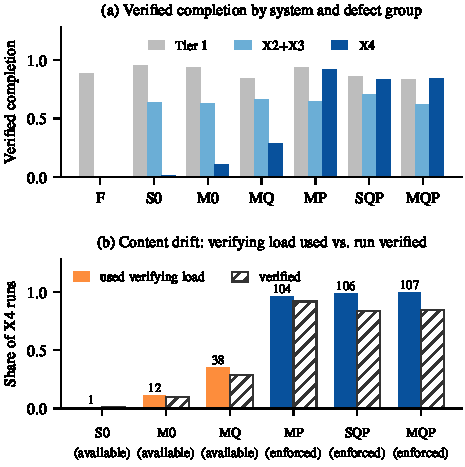
\includegraphics[width=\columnwidth]{figures/fig_main.pdf}
\caption{E1 results. (a) Verified completion by defect group. (b) Verification uptake on X4 (solid bars: orange for available-only verification, blue for provenance-gated agents) versus verified completion (hatched bars). Labels above solid bars are uptake counts out of 108, not completion counts. Calling the verifying load does not guarantee a valid final pipeline.}
\label{fig:main}
\end{figure}

\begin{table*}[t]
\caption{Paired, family-weighted VCR differences in percentage points with individual 95\% block-bootstrap intervals. H1 has an unadjusted primary sign-flip $p$-value; all other $p$-values are Holm-adjusted within the five-test secondary family. ``No X4'' excludes content drift. H4 is defined only on Tier~1.}
\label{tab:contrasts}
\centering\footnotesize\setlength{\tabcolsep}{3pt}
\begin{tabular}{@{}lrrrrr@{}}
\toprule
Contrast & Overall [95\% CI] & $p$ & Tier 1 [95\% CI] & Tier 2 [95\% CI] & No X4 [95\% CI] \\
\midrule
H1: \sys{MQP}$-$\sys{M0} & $+0.1$ [$-11.1$, $+9.9$] & 1.000 & $-10.3$ [$-21.3$, $-0.7$] & $+24.4$ [$+12.3$, $+34.9$] & $-8.1$ [$-19.1$, $+1.4$] \\
Quality main effect & $-6.3$ [$-17.3$, $+3.8$] & 0.50 & $-10.0$ [$-21.1$, $+0.3$] & $+2.2$ [$-9.0$, $+12.0$] & $-7.7$ [$-18.7$, $+2.4$] \\
Provenance main effect & $+6.4$ [$+5.5$, $+7.4$] & $<0.001$ & $-0.3$ [$-1.2$, $+0.5$] & $+22.2$ [$+19.8$, $+24.7$] & $-0.5$ [$-1.4$, $+0.5$] \\
Quality $\times$ provenance & $-4.4$ [$-6.2$, $-2.5$] & 0.013 & $-0.7$ [$-2.5$, $+1.2$] & $-13.0$ [$-18.5$, $-7.4$] & $-2.0$ [$-3.8$, $-0.2$] \\
H3: \sys{MQP}$-$\sys{SQP} & $-3.2$ [$-4.5$, $-1.8$] & 0.041 & $-2.4$ [$-3.8$, $-0.7$] & $-5.2$ [$-8.0$, $-2.5$] & $-3.7$ [$-5.2$, $-2.0$] \\
H4: \sys{MQP}$-$\sys{F} & -- & 0.001 & $-5.4$ [$-7.9$, $-2.5$] & -- & -- \\
\bottomrule
\end{tabular}
\end{table*}

\subsection{RQ1: Verification availability and actual uptake}
Pilot uptake was low: ungated agents used the verifying load in 2 and 5 of 72 content-drift runs. The formal results match that descriptive expectation. On X4, \sys{S0} used the operation in 1 of 108 runs and \sys{M0} in 12, compared with 104, 106, and 107 for \sys{MP}, \sys{SQP}, and \sys{MQP}. Yet completion for these three gated agents was 0.917, 0.833, and 0.843. The gap between uptake and completion shows that checking source contents is necessary for this defect but does not satisfy every pipeline requirement.

Uptake did not increase descriptively in response to X4: the ungated team used the policy in 11.1\% of X4 runs versus 13.1\% on Tier~1, and the single agent in 0.9\% versus 0.4\%. Tier~1 lacks silent content replacement but is not uniformly clean; it includes declared defects. The most frequent first-failure category on X4 was recorded as a wrong source version (105 single-agent and 88 team runs). This diagnostic label should not be confused with a visibly changed catalog version: X4 leaves catalog metadata unchanged.

\sys{MQ} used the verified policy in 38 of 108 runs even though its quality gate cannot detect content drift. Only two uses followed a failed check. This is consistent with an effect of check-related instructions or other configuration differences, but does not isolate prompting as the cause. With backbone B, \sys{M0} never used the policy on X4 (0/18), whereas the gated agents used it in 17/18 and 18/18 runs. Because X4 has no obvious value-level signal, these results primarily measure the background rate of unprompted verification, not recognition of a visible anomaly.

\subsection{RQ2: Overall effect of enforced checks (H1)}
The pilot estimator suggested a positive difference of $+9.2$\,pp. Formal evaluation did not support H1: \sys{MQP}$-$\sys{M0} was $+0.1$\,pp (95\% CI $-11.1$ to $+9.9$; $p=1.0$). The interval permits both meaningful harm and benefit; it is not evidence that the systems are equivalent. The variance-inflated interval ($-13.1$ to $+13.3$) and leave-one-family-out estimates ($-2.3$ to $+4.4$) similarly do not establish an overall gain. The prespecified mixed-effects model gave an odds ratio of 1.01 (0.86--1.19).

The pooled result combines opposing effects: $-10.3$\,pp on Tier~1 and $+24.4$\,pp on Tier~2. The reported decomposition attributes $+7.4$\,pp of the overall contrast to X4 and $-8.3$\,pp to the range-check failure. Plausible ranges were computed from training data and widened by 25\% of each span. In one repetition of D2 and one of D4, valid validation values lay outside those ranges. The quality gate therefore rejected data that the independent evaluator accepted.

Across these two blocks, or 120 runs per system, every quality-gated system had zero verified completions. Most agent runs exhausted their budget attempting repairs: 107 for \sys{MQ}, 109 for \sys{MQP}, and 97 for \sys{SQP}; \sys{F} abstained in every run. Systems without Q verified 75.0--86.7\% of the same instances. The range check nevertheless detected every X3 instance. A rule could therefore be sensitive to the intended unit defect while insufficiently specific for legitimate variation.

Excluding the two blocks \emph{post hoc} yields $+9.3$\,pp (95\% CI $+7.0$ to $+11.4$), falling to $+0.9$\,pp when X4 is also excluded; \sys{F} reaches 1.000 on Tier~1. A post-hoc logistic model with a system slope per block gives an odds ratio of 1.30 (1.05--1.61), allowing block-specific system effects. These analyses describe sensitivity to the false-alarm blocks. They do not replace the frozen primary estimate or demonstrate that a revised gate would achieve the same result.

\subsection{RQ3: Contributions of quality and provenance (H2)}
The expectation that each gate helps with defects it can observe is only partly supported. Provenance has a positive main effect of $+6.4$\,pp (95\% CI $+5.5$ to $+7.4$; Holm $p<0.001$). The benefit is concentrated on X4: $+68.5$\,pp on content drift, compared with $-0.5$\,pp without X4. This supports enforcing source-content agreement in the constructed setting, not a general benefit across every defect type.

The quality main effect is $-6.3$\,pp (95\% CI $-17.3$ to $+3.8$; Holm $p=0.50$). On X3, the fully gated single agent gains 23.1\,pp over its ungated counterpart (95\% CI $+10.2$ to $+35.2$), while the factorial quality effect within the team is $+8.8$\,pp ($-4.2$ to $+20.8$). The first comparison adds both gates, so it is not a pure single-agent Q ablation. Together with the false-alarm blocks, these results show why detecting a targeted defect need not improve aggregate completion.

The interaction is negative ($-4.4$\,pp; 95\% CI $-6.2$ to $-2.5$; Holm $p=0.013$): the joint treatment improves VCR less than an additive combination of the two main contrasts would imply. Neither gate showed a benefit on X2. Pilot traces suggest that many key-variant failures exhausted the budget during exploration, but this observation does not establish the formal-run mechanism for every X2 failure.

\subsection{RQ4: Coordination and rule-based automation (H3, H4)}
The gated team completed fewer verified pipelines than the gated single agent: $-3.2$\,pp (95\% CI $-4.5$ to $-1.8$; Holm $p=0.041$). Mean active time was 223 versus 138\,s per run, approximately 60\% longer; active time excludes waiting for a shared fitting slot. Thus, this three-role design did not convert the common budget ceilings into a reliability advantage. The result is consistent with studies showing coordination overhead under constrained resources~\cite{tran2026single,dylan2026equalcost}, but it does not identify which delegation or communication step caused the difference.

On Tier~1, \sys{F} exceeded \sys{MQP} by 5.4\,pp (95\% CI for \sys{MQP}$-$\sys{F}: $-7.9$ to $-2.5$; Holm $p=0.001$), despite false-alarm abstentions. This supports fixed automation when the required repairs are explicit. Its Tier~2 VCR of zero also shows the limit of that conclusion: the baseline was not programmed to adapt to undisclosed defects. Agents' hidden-defect advantage should therefore not be generalized to superiority over all possible deterministic repair systems.

\subsection{Replication, refusal, and replay}
Backbone B reproduced the primary pattern on six prespecified tasks: H1 was $0.0$\,pp (95\% CI $-12.2$ to $+10.6$), with $-15.9$\,pp on Tier~1 and $+37.0$\,pp on Tier~2. This is a targeted cross-model replication, not a repeat of all 36 tasks. In E5, systems correctly refused 33--36 of 36 unsatisfiable runs each (\sys{F} and \sys{MP} 36, \sys{MQP} 35, \sys{S0}, \sys{M0}, and \sys{SQP} 34, \sys{MQ} 33). All five false submissions involved conflicting authority records, identifying a boundary case for refusal logic.

In E6, all 146 retained submissions reproduced their recorded outcomes and were invariant to row and column order. Forty-five corruption-audit checks in 32 submissions did not return the expected code: in 18 the audit applied no corruption because every numeric column was string-encoded, in 24 (12 submissions) the hash-verifying load correctly avoided the corrupted file because an intact replica existed, and in 3 the corruption was flagged under a different failure code. Outcome replay and corruption-test validity are different checks. The audit exceptions therefore qualify the robustness evidence rather than supporting a claim of universal corruption-test success.

\section{Discussion and Limitations}
\label{sec:discussion}
\subsection{What the results imply}
\textbf{Verification must be evaluated as behavior.} Providing an operation, calling it, and completing a verified pipeline are separate events. RQ1 shows low voluntary use under the tested descriptions; the uptake--completion gap shows that enforcing one check is not sufficient for end-to-end correctness. This parallels the successive verification bottlenecks identified by RITE~\cite{zhang2026rite}, while adding controlled source-content verification in data mining.

\textbf{A check is also a model of acceptable data.} The provenance check has a precise reference: stored bytes must match an authorized hash. The range check instead applies an empirical boundary derived from training data. These rules have different failure risks. A valid observation outside a training-derived interval can become a blocking false alarm, consume repair effort, and eliminate completion. This distinction explains why the provenance benefit and quality losses coexist, and complements work on predicate coverage and interacting controls~\cite{besanson2026sarcdq,besanson2026onegate}.

\textbf{Aggregate scores depend on the defect mix.} X4 is one of ten conditions yet accounts for most of the provenance benefit. Reporting overall VCR alone would obscure that dependence. Tier-specific and no-X4 results make the interpretation more useful: the tested checks are valuable where they observe the relevant violation, but the current evidence does not establish broad protection against arbitrary data defects.

\textbf{Coordination needs a task-specific justification.} The tested team was slower and modestly less reliable than one gated agent. This supports measuring coordination against a strong single-agent baseline, not assuming that more roles imply better checking. Other architectures and decomposable tasks can benefit from collaboration~\cite{fu2026moreagents,kim2025scaling}; the present experiment does not test those alternatives.

\subsection{Validity and reporting limits}
The benchmark measures contract compliance, not unrestricted analytical insight or deployment safety. Explicit contracts and bounded operators simplify discovery relative to open-ended data science. The two synthetic families reduce reliance on public datasets but do not eliminate familiarity with task structures. Six purposively selected families and three repetitions per family limit external validity and precision; thousands of runs do not create thousands of independent dataset-level replications.

Enforcement combines blocking, feedback, and instructions that mention checks. No instructed-but-ungated, advisory-only, or evidence-based override condition was tested. Tool descriptions were fixed, although descriptions can strongly influence selection~\cite{faghih2025toolprefs}. Accordingly, the findings do not isolate enforcement from all communication effects, and low uptake should not be treated as a universal property of every prompting strategy.

Both backbones are approximately 30B-parameter open models used without reasoning mode. The replication includes only six tasks. On X4, hash recomputation is built into the defect's detection mechanism, so provenance gains are close to a manipulation check; the no-X4 contrast is essential to interpretation. The false-alarm blocks were not identified before the freeze because the pilots did not trigger them and the oracle tested solvability rather than gate acceptance. Removing them retrospectively changes the evaluated task set.

Finally, the study reports a one-line type-conversion change to the frozen replay-audit code after a newer pandas version caused an error. No recorded run, outcome, or analysis setting was changed. This maintenance change must remain distinguishable from modifications to the evaluated system. Model candidates and hyperparameters, data splits, seeds, prompts, environment versions, and that patch are in the public repository.

\section{Reproducibility and Ethics}
The frozen protocol is registered and public on OSF (\url{https://doi.org/10.17605/OSF.IO/BN6VA}). The public repository \url{https://github.com/ahsanshahid-1/adm_freeze} contains the frozen package at tag \code{freeze-20261112} with a script that recomputes its hashes, the full source with task generators and seeds, the evaluator, all run records and trusted traces, the final report, and the analysis scripts behind every number in this paper. Software is released under the MIT licence and records and results under CC~BY~4.0. The reported resource use is approximately 23.4 GPU-hours for pilots and 47.5 GPU-hours for formal experiments. The study involves no human participants or personal data and uses neither human nor LLM grading. The failure cases are synthetic benchmark perturbations intended to evaluate reliability, not evidence of misconduct in the source datasets.

\section{Conclusion and Future Work}
This study examined whether LLM agents verify their data when the operation is available and whether enforced quality and provenance checks improve reliability. A paired benchmark combined 36 tasks, declared and hidden defects, seven systems, bounded workflow graphs, and independent hidden-reference evaluation. The 8,352 scheduled runs address all four research questions without supporting the primary claim of an overall benefit from fully enforced checks.

For RQ1, ungated agents rarely used hash verification. For RQ2, the fully gated and ungated teams differed by only $+0.1$\,pp, with a wide interval spanning harm and benefit. For RQ3, provenance checks helped primarily on silent content drift, while quality checks detected undeclared units but also rejected correct data. For RQ4, the tested team underperformed the gated single agent, and fixed automation performed better on declared repairs. These results identify verification uptake, predicate validity, and coordination cost as distinct issues rather than a single measure of agent capability.

Future work should separate prompting, diagnostic feedback, and blocking in controlled ablations. Advisory checks could warn about unusual but plausible values; evidence-based overrides could require an agent to justify an exception without bypassing source-integrity requirements. Range thresholds could be calibrated on held-out data and evaluated for both defect detection and false rejection before enforcement. Broader datasets, additional repetitions, larger or reasoning-enabled models, and alternative team designs would test the scope of the current findings. These are proposed extensions, not evaluated improvements. The central lesson is that reliable agentic data mining requires not only accessible verification tools, but checks that agents use and whose decisions are themselves justified.

\section*{Acknowledgment}
Research supported by the NVIDIA Academic Grant Program using an NVIDIA RTX PRO 6000 Blackwell Max-Q Workstation Edition GPU. This research was partially supported by the National Science Foundation under EPSCoR Award No.\ OIA-1946391.

\textit{Use of AI tools.} An IDE-based AI coding assistant using Anthropic Claude Opus~5.5 was used to help write the study software, run and monitor the experiments, write the analysis scripts, and draft and edit the text of all sections. OpenAI ChatGPT was used in a later revision to improve language, organization, and LaTeX formatting, and to check bibliographic entries. The authors directed the research, reviewed all AI-assisted material, and take full responsibility for the methods, analysis, interpretation, and results.

\bibliographystyle{IEEEtran}
\bibliography{refs}
\end{document}
